%% LaTeX Beamer presentation template (requires beamer package)
%% see http://bitbucket.org/rivanvx/beamer/wiki/Home
%% idea contributed by H. Turgut Uyar
%% template based on a template by Till Tantau
%% this template is still evolving - it might differ in future releases!

%% Template edited by Panagiotis Adamopoulos {padamopo}@stern.nyu.edu

\documentclass{beamer}
 
\mode<presentation>
{
\usetheme{NYU}

\setbeamercovered{transparent}
}

\usepackage[english]{babel}
\usepackage[latin1]{inputenc}

% font definitions, try \usepackage{ae} instead of the following
% three lines if you don't like this look
\usepackage{mathptmx}
\usepackage[scaled=.90]{helvet}
\usepackage{courier}

\usepackage{float}
\usepackage{wrapfig}


\usepackage[T1]{fontenc}

\usepackage{comment}
%usepackage{appendixnumberbeamer}
%\usepackage{amsmath}
\usepackage{pgfpages}
% citations

\usepackage{natbib}
\bibliographystyle{unsrtnat}
\bibpunct{(}{)}{;}{a}{,}{,}
\def\citeapos#1{\citeauthor{#1}'s (\citeyear{#1})}
\renewcommand{\bibsection}{\subsubsection*{\bibname } }
\graphicspath{ {images/} }


\title{Quality Assurance In Microservice Architectures}

%\subtitle{}

% - Use the \inst{?} command only if the authors have different
%   affiliation.
%\author{F.~Author\inst{1} \and S.~Another\inst{2}}
\author{Krishnan Chandran \and Irina Barykina} 

% - Use the \inst command only if there are several affiliations.
% - Keep it simple, no one is interested in your street address.
\institute[NYU]
{
Department of Informatics,\\
Intelligent Adaptive Systems, UHH\\
}

\date{2016}


% This is only inserted into the PDF information catalog. Can be left
% out.
\subject{Subject}



% If you have a file called "university-logo-filename.xxx", where xxx
% is a graphic format that can be processed by latex or pdflatex,
% resp., then you can add a logo as follows:

% \pgfdeclareimage[height=0.5cm]{university-logo}{university-logo-filename}
% \logo{\pgfuseimage{university-logo}}



% Delete this, if you do not want the table of contents to pop up at
% the beginning of each subsection:
%\AtBeginSubsection[]
%{
%\begin{frame}<beamer>
%\frametitle{Outline}
%\tableofcontents[currentsection,currentsubsection]
%\end{frame}
%}

% If you wish to uncover everything in a step-wise fashion, uncomment
% the following command:

%\beamerdefaultoverlayspecification{<+->}

\begin{document}

\begin{frame}
\titlepage
\end{frame}

%\begin{frame}
%\frametitle{Outline}
%\tableofcontents
% You might wish to add the option [pausesections]
%\end{frame}

%==============================Start
% Theory section
\section{Structure}
%\subsection[Short First Subsection Name]{First Subsection Name}
\begin{frame}
	\frametitle{Structure}	
	\framesubtitle{}
	Goal: explore QA techniques and approaches, that could cope with challenges specific for microservice architectures. \\
	Structure:
	\begin{itemize}
		\item Give an insight of why QA is important and what challenges it meets in microservice architectures. 
 		\item Give and overview of QA techniques that are used in all stages of development: from coding phase to production. Explain benefits that we gain, using these 	   techniques. 
		\item Show on the example of metasearch engine how these techniques could be applied and how they could be adapted to different scenarios.
		\item Provide some examples of software tools and show how they could be used for an implementation of explored QA techniques.
	\end{itemize}
\end{frame}

\section{Theoretical part}
\begin{frame}
	\frametitle{Theoretical part}	
	\framesubtitle{}

	\begin{itemize}
 		 \item Challenges of testing in microservice architectures.
		 \item Types of tests (Cohn Test Pyramid), their purposes, scopes and quantities. Ice Cream Cone antipattern.
		 \item Non-functional testing: performance, security.
		 \item Rapid application deployment as a prerequisite for microservices. Deployment pipeline. Continuous integration, deployment and delivery.
		 \item Releasing strategies: blue/green deployment, canary releasing, smoke tests.
		 \item After release quality assurance: monitoring, DevOpsCulture. 
	\end{itemize}
\end{frame}
%===============================End

%==============================Start
% Scenarios section
\section{Example}
\begin{frame}
	\frametitle{Example}
	We are going to use an example of metasearch engine (for traveling-related information) throughout our presentation to show how explored techniques could be applied. 
	We also want to show that testing strategies should be adapted to concrete scenarios on the example of:
	\begin{itemize}	
 		\item Scenario 1: Testing microservices within application.
		\item Scenario 2: Testing microservices that use third-party service
		\item Scenario 3: Testing microservices that will be or is already exposed to public domain
	\end{itemize}
\end{frame}
%===============================End


%==============================Start
% Tools section
\section{Tools}

\begin{frame}
	\frametitle{Tools}
	\framesubtitle{}
	\begin{itemize}
		% Unit testing: Unit testing is a testing of smallest testable parts of applications, ideally of single methods or procedures. Unit testing helps to identify bugs on
		% the early stages and most precisely (up to the line of code).  Unit testing is also the powerful designing tool (especially if it is used in the context of TDD),
		% because it highlights when module should be broken into smaller more coherent pieces.
		\item xUnit framework
		\item stubbing and mocking (on the example of Mockito)
		\item smart stubbing with Mountebank
		\item testing of data passing between services (on the example of SOAP UI)
		\item consumer driven testing (on the example of Pact)
		\item End-to-End Testing (BDD Tools, JBehave, Cucumber)
	\end{itemize}
\end{frame}

%===============================End

%===============================Start
% CD related slides
%===============================End
\section{Deployment}

\begin{frame}
	\frametitle{Deployment}
	\framesubtitle{RAD and Deployment Pipeline}

\end{frame}

\begin{frame}
	\frametitle{Deployment}
	\framesubtitle{Continuous Deployment and Delivery}

\end{frame}

\begin{frame}
	\frametitle{Deployment}
	\framesubtitle{DevOps Culture}

DevOps Culture:
	\begin{itemize}
		\item Aim: break silos between development and later stages 
		\item Requirements: shared responsibility and autonomy of teams
	\end{itemize}
	\begin{figure}
		\begin{center}
% image is from http://blogs.atlassian.com/2016/03/how-to-choose-devops-tools/
% reference it!
 			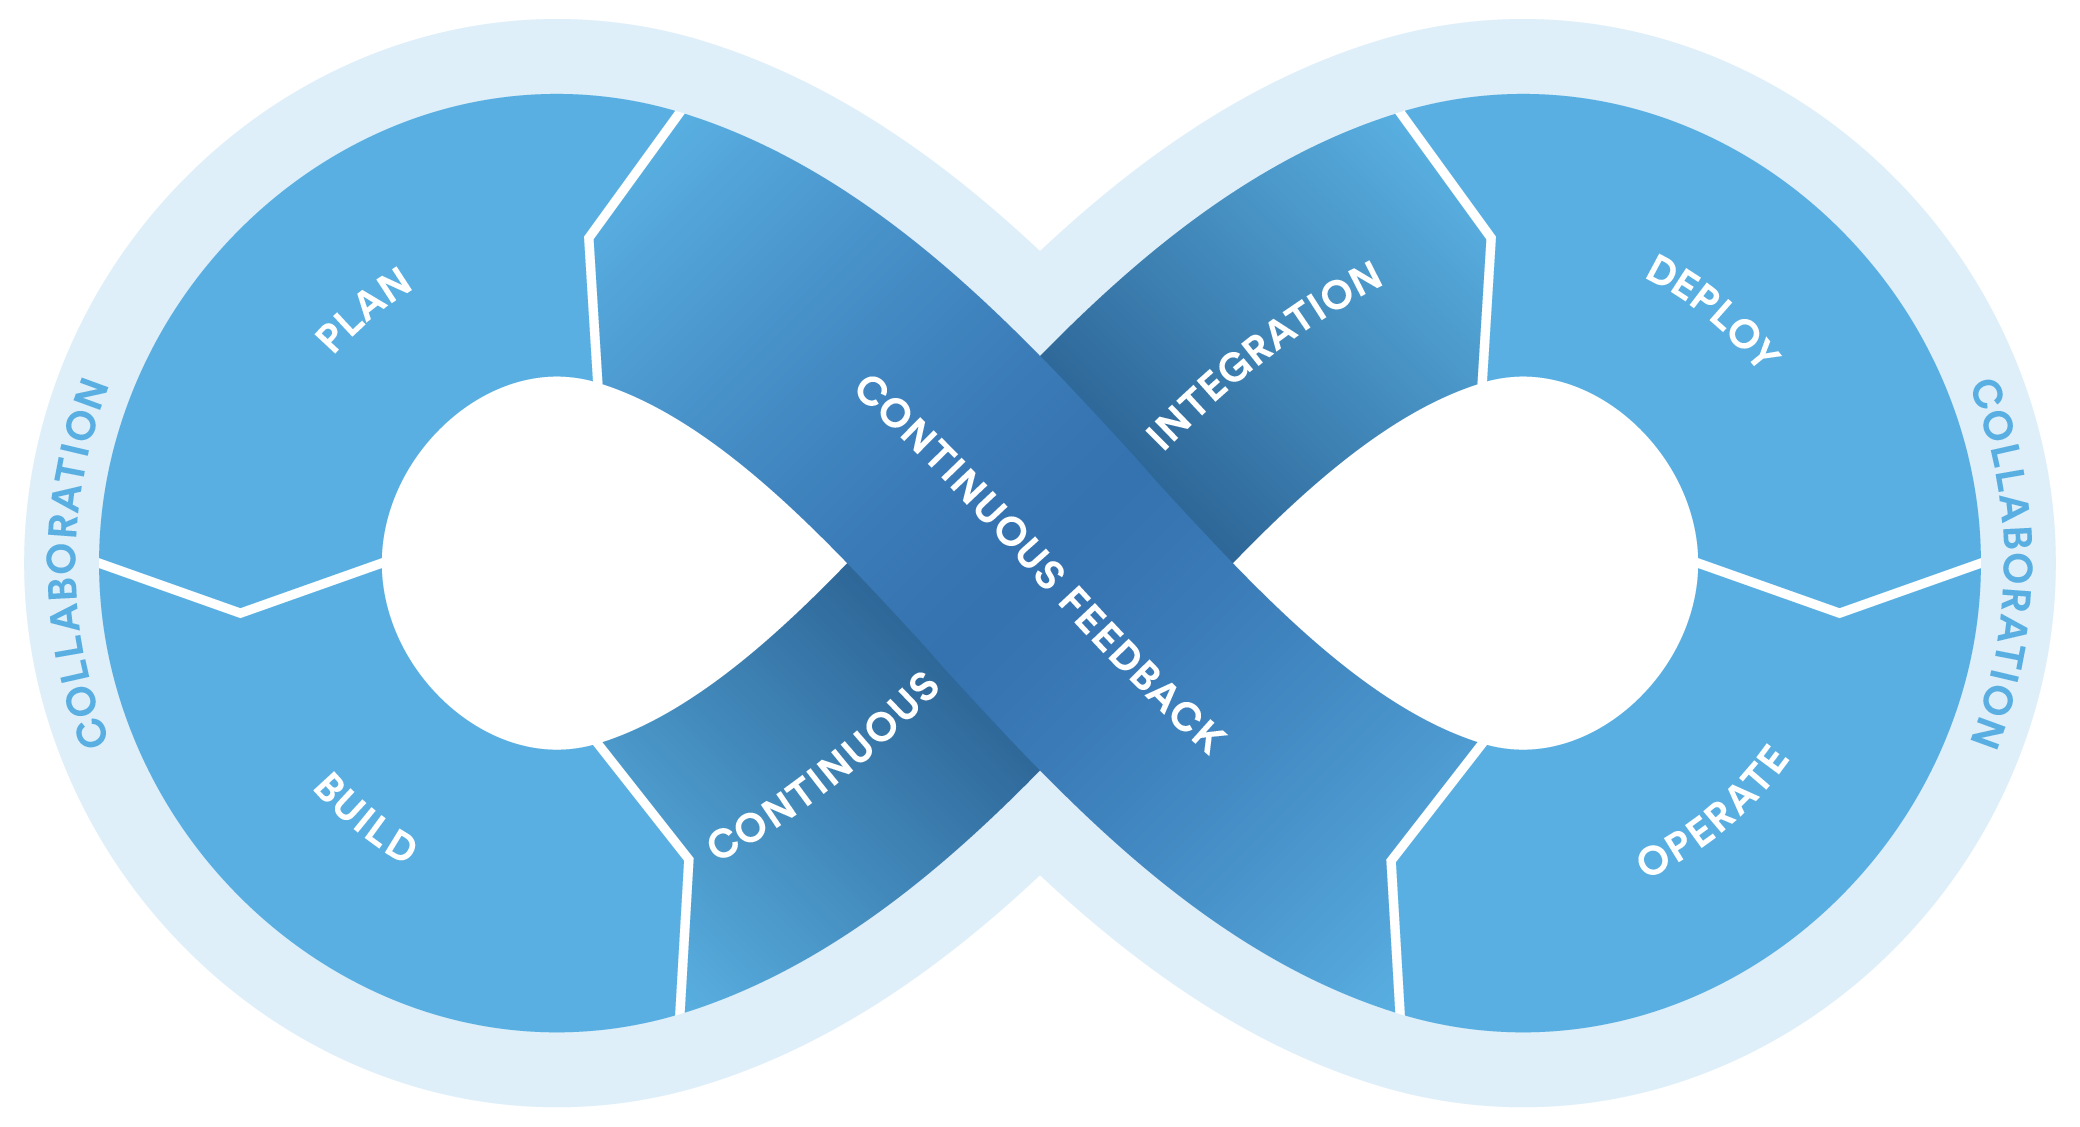
\includegraphics[scale=0.12]{devopsloop}
		\end{center}
	\end{figure}

\end{frame}


%===============================Start
% Smart releases slides
%===============================End
\section{After Deployment}

\begin{frame}
	\frametitle{After Deployment}
	\framesubtitle{Smart releasing strategies}
\begin{columns}
 \begin{column}{.49\textwidth}
	\begin{itemize}
		\item Smoke Test Suites
		\item Blue/Green Deployment
		\item Canary releasing
	\end{itemize}
\end{column}
\begin{column}{.49\textwidth}
	\begin{figure}
		\begin{center}
 			\only<1>{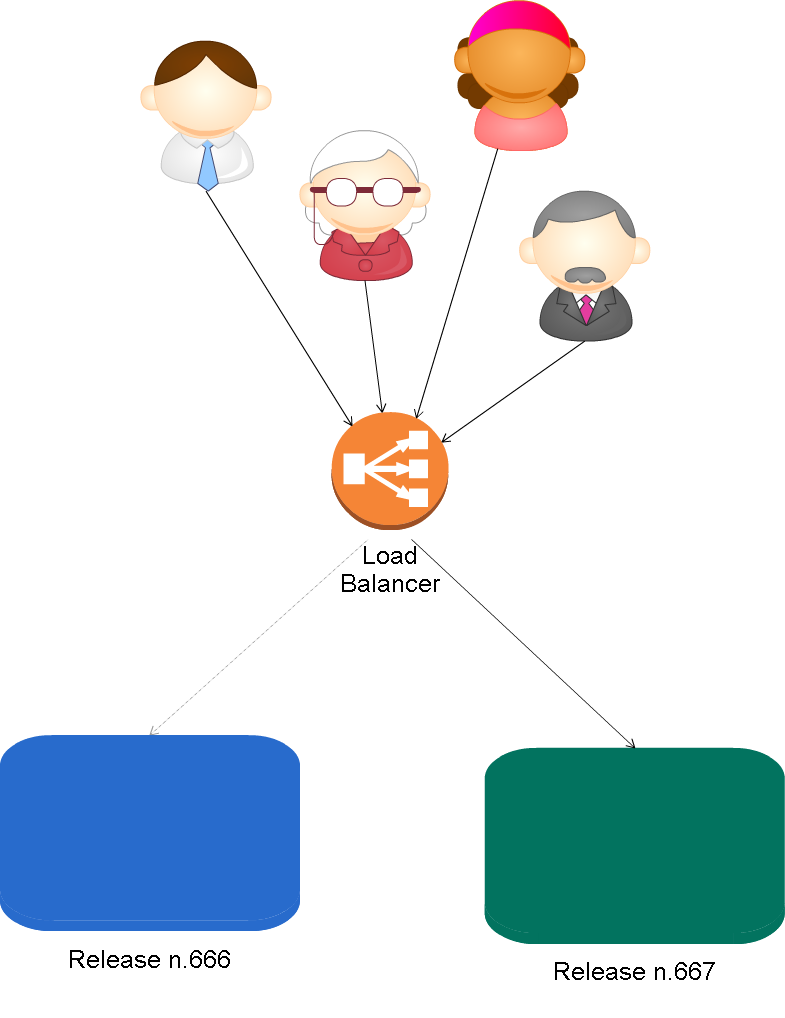
\includegraphics[ scale=0.16]{blue_green}\\}
 			\only<2>{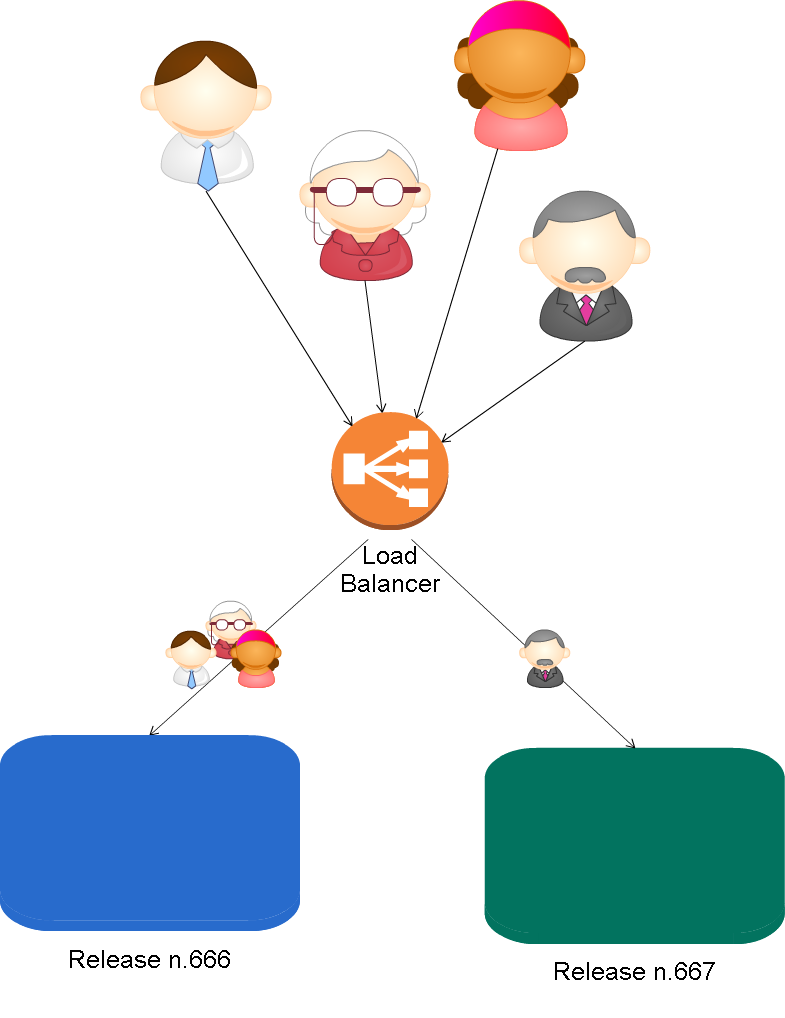
\includegraphics[ scale=0.16]{canary}}\par
		\end{center}
	\end{figure}
\end{column}
\end{columns}
\end{frame}

\begin{frame}
	\frametitle{After Deployment}
	\framesubtitle{Monitoring}
\end{frame}


%==============================Start
% References section
\section{References}
\begin{frame}
	\frametitle{References}
	\framesubtitle{}

	% make a list even without citation
        \nocite{newman,cohn,infosys,clemson,fowler_cont_del,naik}
	\bibliography{references}
\end{frame}

%===============================End


\end{document}
